\documentclass[12pt]{article}
\usepackage{lingmacros}
\usepackage{tree-dvips}
\usepackage{graphicx}
\usepackage{authblk}

\title{Coloração Propria: um estudo aprofundado}
\author{Autores: Gabriel Souza, Jonathan Melo}
\affil{Orientador: Prof. Celso Aimbiré Weffort Santos }
\date{06 de Abril, 2020}

\begin{document}
	
	\maketitle
	
	
	\section{Introdução}
	Nesta seção será mostrado os conceitos iniciais sobre grafos, os objetivos procurados durante a pesquisa sobre o tema, a justificativa para o tema escolhido, bem como a notação que será usada durante o documento para a descrição dos conceitos.
	
	\subsection{Informações gerais sobre grafos e sua história }
	
	A ideia inicial do que hoje se tornou um dos grandes estudos da área da matemática e tecnologia partiu de Leonhard Euler (1707 –1783) matemático e físico suíço que teve sua motivação para a criação do problema das Sete Pontes de Königsberg.
	
	\subsubsection{As Sete Pontes de Königsberg }
	
	A cidade de Königsberg (após 1946 chamada de Kaliningrado) é uma cidade russa onde em uma parte do seu território existe um rio que separa a cidade em duas áreas. No decorrer desse rio existiam 7 pontes conectando as duas áreas da cidade formando algo parecido com esta imagem:

 
{\centering  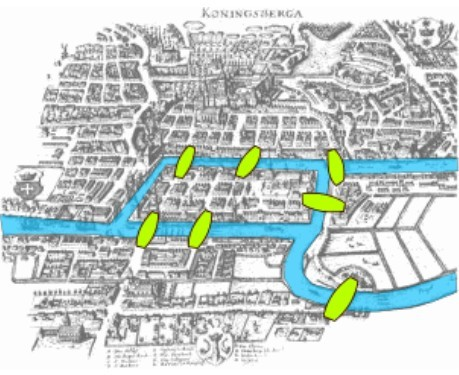
\includegraphics[width=8cm, height=8cm]{pontesKonisberg}\par}   


    Figura 1: Mapa das pontes de Königsberg
   
    A motivação de Euler veio a partir de uma discussão feita pelos moradores da cidade, os mesmos argumentavam se era ou não possível atravessar todas as pontes sem repetir nenhuma delas durante o trajeto.
   
   Euler provou que era impossível este trajeto e deu início ao primeiro teorema da teoria de grafos, antes de introduzirmos os termos técnicos, se fossemos trazer este teorema para o problema das pontes, Euler provou que para que esse caminho fosse possível, cada uma das regiões do mapa precisaria ter um número par de pontes incidentes a ele. O teorema descrito, levou o nome de Ciclo Euleriano.
   
   Após criado o conceito inicial sobre grafos criado por Euler, um outro matemático introduziu uma nova forma de desenharmos um grafo, William Thomas Tutte (1917-2002) definiu que um grafo poderia ser representado por vértices(pontos) e arestas(linhas), aonde os vértices são interligados por arestas conectados a eles, trazendo esta definição para o problema das sete pontes, definiríamos que ponte do mapa seria uma aresta e cada ilha seria um vértice, tendo sua definição visual parecida com a imagem a baixo.
   
   {\centering  \includegraphics[width=6cm, height=6cm]{grafoKönigsberg}\par} 
   
   Figura 2:  Representação do grafo das sete pontes de Königsberg
   
   	\subsection{Conceitos técnicos da teoria de Grafos}
   	
   	Como vimos na seção anterior, após as descobertas de Euler, foram introduzidos novas maneiras de lidarmos com problemas parecidos.
   	Um grafo G é composto por vértices (V) e arestas (E) sendo sua composição completa denotada como G (V, E). O número de vértices contidas em um grafo é definido como a Ordem do grafo (N) e o número de arestas é o seu Tamanho (M). Esses conceitos iniciais sobre o tema, podem ser desdobrados em outros conceitos que complementam e inserem novas definições para o grafo.
   	
   	\subsubsection{Vizinhança de vértices}
   	
   	Em um grafo G existem os vértices U e V ligados por uma aresta de G, baseado nessas afirmações podemos definir que os vértices U e V são adjacentes ou vizinhos, caso em nosso grafo existissem mais duas vértices ligadas a vértice V sendo elas Z e W, poderíamos a partir disso definir que a vizinhança de V é: N (V) {U, Z, W}. 
   	
   	\subsubsection{Grau de vértices}
    Em um Grafo G contendo os vértices V (U, X, W) e as seguintes vizinhanças de vértices N(U) {X, W}, N(X) {U} e N(W) {U}, definimos que o grau de um vértice é o número de arestas incidentes nele e é denotado como d(v), baseado nessa condições e utilizando o exemplo criado, denotaríamos o grau de U como D(U)=2, D(X) = 1 e D(W) = 1, visto que baseado em nossa vizinhança esse é o número de arestas incidentes em cada um de nossos vértices.
    Dentro da definição do grau de um grafo existem as notações a serem usadas para 
    
    \subsection{ Coloração própria de vértices em grafos}
    Sendo esse o tema escolhido para as nossas pesquisas, a definição do problema diz que para termos uma coloração própria dentro de um grafo, vértices que são adjacentes não podem ter a mesma cor. Desta maneira podemos definir também um número cromático para o nosso grafo denotado de x(G), número esse que é definido como o menor número de cores possíveis para pintar um grafo de forma que cumpramos odas as regras definidas para um grafo com coloração própria.
    Um grafo G é considerado k-Colorivel, se pudermos dentro dele usar um número K de cores para sua coloração sem que afetemos a regra da coloração própria.
    
    \subsubsection{História e o problema das quatro cores}
    
    Antes de introduzirmos a motivação para o problema da coloração própria, é preciso definir o conceito de um grafo planar, visto que este tipo de grafo foi a motivação inicial para a criação da primeira definição da coloração própria de grafo.
    Um grafo G é considerado planar se puder ser desenhado no plano sem que nenhuma de suas arestas se cruzem, exemplo de um grafo planar na imagem abaixo:
    
    {\centering  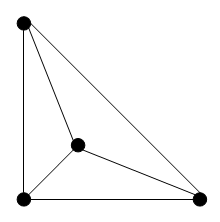
\includegraphics[width=5cm,height=5cm]{grafoPlanar}\par} 
    
     Figura 3:  Exemplo de grafo planar
     
    A primeira ideia de co'loração própria se deu em 1852 aonde o matemático Francis Guthrie criou a teoria que para todo mapa o número mínimo de cores necessárias para pinta-lo para que nenhuma de suas regiões que partilhassem fronteiras fossem pintadas da mesma cor era sempre quatro.
    
   
    Em 1879 Alfred Bray Kempe publicou a primeira suposta solução para a teoria das quatro cores, solução essa que foi considerada incorreta por Percy Heawood em 1890, que também foi o criador do teorema das Cinco cores, e provou a veracidade do mesmo.
    
    Apesar de ser considerado incorreta a teoria de Kempe, ela foi grande influenciadora para que em 1977 Kenneth Appel (1932-2013) e Wolfgang Haken(1928) com o auxílio do uso de um computador, provaram novamente que a teoria das quatro cores era correta.
    
    Os mapas estudados por esses matemáticos são considerados mapas que podem ser representados por um grafo, o nome que esse grafo leva é de grafo dual. 
    
     {\centering  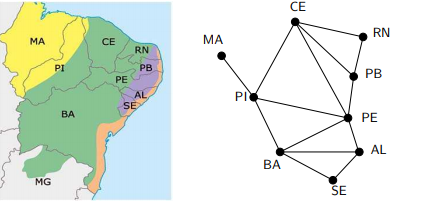
\includegraphics[width=8cm,height=4cm]{grafoDual}\par}
   	
   	Figura 5: Exemplo de grafo Dual
   	
   	\subsubsection{Complexidade da solução}
   	
   	Nos problemas envolvendo coloração própria de vértices, encontrar um número K de cores possíveis é relativamente fácil, visto que se tivermos N vértices podemos ter que K = N e ter uma cor para cada vértice do grafo. A maior dificuldade para este tema é encontrar o número cromático da instância ou o menor número de cores possível, transformando este tema em um problema computacional extremamente difícil aonde validar uma solução é muito fácil porém achar uma solução se torna muito difícil.
   	Validar uma solução como citado acima nos casos de coloração própria é fácil pois baseado na instancia que nos foi dada, podemos validar todos os vértices adjacentes a ele de forma rápida, validando se eles tem ou não a mesma cor. Já para criarmos uma solução isso se torna extremamente difícil, dado um grafo G aonde V(G) = {V1, .... Vn }, para encontrar a solução com o melhor número cromático desta instancia devemos validar todas as situações e adjacências de todos os vértices do grafo, para isso normalmente são utilizados algoritmos de busca que serão citados e explicados posteriormente.
   	
   	\subsubsection{Aplicação reais do tema}
   	
   	Neste tópico iremos descrever algumas aplicações no nosso dia aonde o auxílio do conceito de coloração própria de grafos seria útil para encontrarmos a melhor solução para o problema escolhido.
   	
   \title{Organização de provas de uma universidade}
   
   \subsubsection*{1.3.3.1 Organização de provas de uma universidade}
  
   Um dos melhores de exemplo do uso da coloração própria em aplicações reais é na organização de provas de uma universidade aonde é necessário que duas disciplinas que contiverem alunos em comum não podem ter suas provas agendadas no mesmo horário, levando-nos a seguinte pergunta, qual seria o menor número de horários que a universidade teria de usar para aplicar todas as provas respeitando as regras da instancia?
   
   
   \subsubsection*{   1.3.3.2 Organizações de produtos químicos em uma indústria}
  
   Em uma indústria química existem N produtos, aonde muitos deles compartilham o mesmo tipo de composição, produtos esses que não podem ser colocados juntos devido a possibilidade de que uma reação química estragassem os mesmos. Baseado nessa instancia, qual seria o menor número de compartimentos possíveis para guardar esses produtos de forma que produtos com a mesma composição não podem ser colocados juntos.

	\subsubsection{Algoritmos de coloração conhecidos}
	
	Nesta seção iremos mostrar conceitos de algoritmos conhecidos que auxiliam na obtenção da melhor solução para uma instancia de coloração própria, visto que a complexidade deste problema é extremamente difícil, a maioria de seus algoritmos são baseados na premissa da busca incansável, aonde iremos executar todas as situações da instancia a fim de no final separar a melhor delas.
	
\subsubsection*{1.3.4.1 Algoritmo de força bruta}
 Dado um grafo G simples aonde V(G) {V1, ... VN, o algoritmo de força bruta com o objetivo de buscar um k-coloração iria verificar cada uma das Kn atribuições possíveis verificando se cada uma delas está correta. Em uma instancia pequena do problema, o algoritmo de força bruta encontraria o resultado de forma relativamente rápida, porém se consideramos que quanto maior a instância do problema maior seria a quantidade de atribuições que deverão ser testadas, esse algoritmo se torna inutilizável e computacionalmente inviável.
 	
 \subsubsection*{1.3.4.2 Algoritmo Guloso}
 	
 	O algoritmo guloso é aquele que faz sempre a melhor escolha local minimizada, esperando que essa escolha se torne também a melhor escolha em um estado global da instancia do problema.
 	Este algoritmo sempre irá trazer a solução para o problema, porém esta solução não necessariamente é a melhor possível, e sim a melhor que o algoritmo encontrou dado as suas condições de busca.
 	
 	 
  \subsubsection*{1.3.4.3 Algoritmo de Welsh-Powell}
  
  Criado em 1975 é um algoritmo guloso que visa a obtenção inicial do grau de cada vértice do grafo e ordenação dos mesmos em ordem decrescente do seu grau. Dado essa ordenação será associado uma cor para o primeiro vértice da lista de vértices ordenados, e também aos próximos vértices da lista que não são adjacentes aos vértices já coloridos com a primeira cor selecionada. Será feito este mesmo processo para os próximos vértices que ainda não foram coloridos, porém agora usando a próxima cor.
  
  \subsection{Objetivos}
  
  O tema dessa pesquisa é muito amplo e completo, de forma que seus conhecimentos se desdobram em várias áreas da ciência da computação e matemática, o objetivo deste projeto é que com o estudo teórico e técnico de várias técnicas e conceitos já criados anteriormente que avançam constantemente o estudo do tema atualmente.
  Estes estudos serão de grande influência para o nosso desenvolvimento matemático e computacional, visto que todas as técnicas até hoje criadas se desdobram dessas teorias, sendo esse o principal objetivo do projeto.
  
  
  \section{Materiais e métodos}
  
  
  
  \section{Resultados esperados}
  Para os resultados esperados ao longo da nossa pesquisa, é esperado que desenvolvamos conhecimento e desenvoltura na área da matemática aplicada, que se desdobra nos estudos da teoria de grafos e consequentemente no estudo e aprofundamento das técnicas e teorias da coloração própria e seu estado de arte.
   
\end{document}
	
